\documentclass[journal,onecolumn]{IEEEtran}
%
% If IEEEtran.cls has not been installed into the LaTeX system files,
% manually specify the path to it like:
% \documentclass[journal]{../sty/IEEEtran}


% Some very useful LaTeX packages include:
% (uncomment the ones you want to load)

\usepackage{placeins}
\usepackage{color}
\usepackage{float}
\usepackage{booktabs}
\usepackage{pgfplots}
\usepackage{graphicx}
\usepackage{caption}
\usepackage{subcaption}
\usepackage{wrapfig}
\usepackage[hidelinks]{hyperref} % Clickable links in PDF.
\usepackage[margin=2.5cm]{geometry}
\usepackage{titlesec}

\newlength\figureheight 
\newlength\figurewidth\scshape


\titleformat{\section}
{\normalfont\Large\bfseries\scshape\centering}{\thesection}{1em}{}
\titleformat{\subsection}
{\normalfont\large\bfseries\scshape}{\thesubsection}{1em}{}
\titleformat{\subsubsection}
{\normalfont\normalsize\bfseries\scshape}{}{1em}{}

% Set sizes figures (all the boxplots in 1 go!)
\setlength\figureheight{0.3\textwidth}
\setlength\figurewidth{0.4\textwidth}

\graphicspath{{./Figure/}}

% FOR CAPTION CENTERING NOT IN LINE WITH THE IEEETRAN STYLE!
%\usepackage{caption}% http://ctan.org/pkg/caption 


\usepackage[cmex10]{amsmath}



\begin{document}

\title{\LARGE Comparing deep neural network architectures for automatic colorization of greyscale images.}

\author{J.L. Dorscheidt (4091981), Dawud Hage (4190696), Dennis van der Hoff (4139925), Joost Meulenbeld (4103548)}% <-this % stops a space
% make the title area
\maketitle

% As a general rule, do not put math, special symbols or citations
% in the abstract or keywords.
%
\begin{abstract}
Automatic colorization of grayscale images with no further user input has several interesting applications, of which grayscale video may be the most useful one. In this paper a comparison is made between several techniques for automatic colorization, all of them being convolutional neural networks. The color space which is used during colorization is found to have an influence on the end result, and CIELab is chosen as the most promising one. Colorization can be seen as a mapping between a grayscale input image and an output color per pixel. While viewing this as a regression problem yields satisfactory results, it is found that implementing it as a classification problem, with the output of the network being a probability distribution over the colors in a discretized color space, yields much better results. The averaging problem, which causes networks to tend towards undersaturated or sepia tones, is shown to be solved using the classification approach. Using an annealed mean with a parameter setting for picking either the mean or mode of the probability distribution yields very convincing results. Finally, a model architecture using dilated convolutions in the upscale reconstruction pipeline of the network is found to generate the most convincing colorization.


\end{abstract}


% For peerreview papers, this IEEEtran command inserts a page break and
% creates the second title. It will be ignored for other modes.
\IEEEpeerreviewmaketitle


\section{Introduction}\label{sec:into}
\IEEEPARstart{I}{n} this paper a deep neural network approach to colorize greyscale images is introduced. Although often automization is already applied on colorization of black and white images, the existing alghorithms still require a lot of input from a user. This paper introduces an algorithm based on a deep neural network architecture that can fully colorize images without the input of a user. High quantities of training data are easily generated by converting RGB images to greyscale for the input and converting to LAB colorspace for the output. 
\section{Literature review} \label{sec:litreview}
%Lit. review (actually previous attempts)
%VGG16
%Dahl
%batch norm
%concatenation
%Zhang
%dilation
%classification


In recent years, Convolutional neural networks (CNN) have become the standard in image
classification \cite{Krizhevsky}. Using a CNN for image colorization is a trend that has emerged only in the past year in the machine learning community. Research from Dahl \cite{Dahl}, Zhang et al. \cite{Zhang}
and Cheng et al. \cite{Cheng} has shown promising results using CNN, however they all use very different
architectures. One of the problems in the image colorization task is the maintainability of spacial information, going back from global features to a special mapping of these features in the detailed image space. 

The use of max-pooling in CNN's makes the network invariant to spatial transformations. However a lot of this information is lost when the final layer of a conventional CNN is reached, which is disadvantageous for a classification and localization task. Different techniques have been proposed to regain a local mapping of the features in the final layers of the network. 

Another big variation lies in the loss function of the research mentioned previously. Dahl \cite{Dahl} and Zhang et al. \cite{Zhang} both use pre-trained networks for the feature mapping such as VGG16 \cite{Simonyan}, however Cheng et al. \cite{Cheng} completely trains the front-end module of the network from scratch. This offers more flexibility with network architecture, however a lot more computational power is required. 

In this section a short summary of the related work on image colorization using CNN is shown. In addition the paper by \cite{Simonyan} on VGG16 is explained.

\subsection{Dahl}

\begin{wrapfigure}{R}{0.42\textwidth}
	\vspace{-20pt}
	\begin{center}
		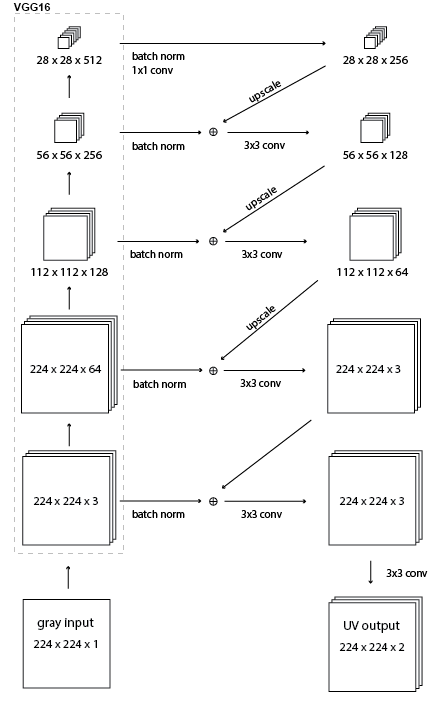
\includegraphics[width=0.42\textwidth]{Dahl_Architecture.png}
	\end{center}
	\caption{Network used by Dahl \cite{Dahl}}
	\label{fig:dahlnetwork}
\end{wrapfigure}


Dahl \cite{Dahl} is one of the first to use a CNN for image colorization. The network is trained in the YUV colorspace, with the advantage that Y-channel can be used directly as the input of the network. Only the U and V channels will be computed by the network and they are concatenated with the original Y-channel, resulting in a colorized image. This way less information needs to be generated by the network. It is unclear whether the network uses exclusively information from semantic features as opposed to learning color distributions coupled to Y inputs. Zhang et al. \cite{Zhang} has shown in their network design that this is not the case. 

The pre-trained VGG16 network is used, which already has a large variety of feature extraction. The network is trained on the ImageNet LSVRC 2012 Training Set. 

Maintaining the spatial information is done with the use of partial hypercolumns, also called a residual auto-encoder \cite{hariharan2015hypercolumns}. The image is upscaled by a factor two after each convolutional layer in the output pipeline of the network. These upscaled feature maps are concatenated with the corresponding input layer's feature maps as can be seen in figure \ref{fig:dahlnetwork}. This combination of global and more local features are then convolved using 3x3 convolutional kernels, this process is repeated until all the layers in the front-end are concatenated with the more global features. 

Batch Normalization was applied after each convolutional layer block towards the concatenate layers (see section \ref{sec:batch_norm}). 
Throughout the network 3x3 convolutional kernels and rectified linear units (ReLu) \cite{nair2010rectified} as non-linearities are used. The loss function consists of calculating the sum of the squared euclidean distances between the target pixel values and the output of the network. 
Gaussian blur is used over the target output of the image, resulting in better guidance of learning. 

One of the problems encountered is that of color averaging, for images which have a large variety of color probabilities the network chooses the average of these colors. For example, cars can have a large variety of colors. 
The network colorizes these cars with the mean of all these colors, so in most cases cars will be colored sepia-like. It is proposed to use generative adversarial networks \cite{Radford}, to counter the color averaging problem. 
Another method to tackle this problem are variational Auto-encoders, altering a direct copy of the output, (variational) auto encoders are described by \cite{Gregor}, \cite{Kingma} and \cite{GoodfellowBOOK}. 


\subsection{Zhang et al.}
Very promising results are obtained by Zang et al. \cite{Zhang}, therefore a lot of the work in this paper is based on their work.
A fully automatic approach is proposed that produces vibrant and realistic colorizations. Again VGG16 is used for feature extraction with some modifications on the input layers. The max-pooling operation is replaced by strides, resulting in less loss of spatial information. 

In the output pipeline of the network, dilated convolutions \cite{yu2015multi} are applied, creating an exponential increasing depth of field with the same number of convolutions compared to conventional convolutional kernels (see figure \ref{fig:dilations}).

\begin{figure}[h]
	\centering
	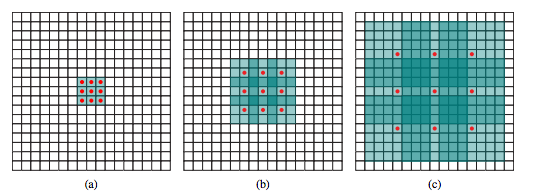
\includegraphics[width=0.63\textwidth]{Dilations}
	\caption{Illustration of dilated convolutions. Figure c shows a receptive field of 15 after only 3 convolutions. Normal convolutions would have a receptive field of 7 after 3 convolutions \cite{yu2015multi}.}
	\label{fig:dilations}
\end{figure}

In addition, the problem is posed as a classification problem, where each output pixel is classified as a certain color. This creates the opportunity of implementing class-rebalancing.
Categorical cross-entropy is applied on the final softmax output layer of the network \cite{de2005tutorial}. The final loss consists out of the categorical cross-entropy loss multiplied with a value function based on the probability of the target color given in equation \ref{eq:lossZhang}, where $H$ and $W$ are the pixel width and height respectively, $Z$ is the target vector, $\widetilde{Z}$ is the output vector, and $v$ is the value function.
Colors which are common in the dataset get a low loss, and colors which are rare in the dataset get a high loss, causing the network to 'steer' towards more saturated colors instead of sepia. 

\begin{equation}
L(\widetilde{Z},Z)=-\frac{1}{HW}\sum_{h,w}v(Z_{h,w})\sum_q^{}{Z_{h,w,q}log({\widetilde{Z}_{h,w,q}})}
\label{eq:lossZhang}
\end{equation}

The colorspace used is CIELab, The L (luminosity) layer is the network input. The CIELab colorspace is discretized into 313 colorbins. Target probabilities per pixel are generated by applying a Gaussian blur on the k-nearest neighbor colorbins. The output of the network consists out of the distribution of probabilities over the colorbins. In order to generate a final choice of colorbin from this output vector, an annealed mean operation is applied on the output probabilities. The temperature T in the annealed mean operation determines whether the mode or the mean of the final distribution is taken as final color. An illustration of the effect of the annealed mean temperature T can be seen in fig \ref{fig:anmean} This operation is described in more detail in section \ref{sec:method}.

Various performance measures were applied by Zhang et al, the most interesting one being a 'Turing test' where participants needed to choose between a fake colorization of the image and the true ground colors of the images. The results of Zhang et. al fooled participants in 20.4 \%\ of the cases. 



\subsection{Iizuka et al.}
Recently the paper by Iizuka et al. \cite{IizukaSIGGRAPH2016} is published where they proposed a network that simultaneously classifies and colorizes the images. Their network shows very promising results. The classification is done to extract the global features of the image, i.e. if the image was taken indoors or outdoors. That is done by a CNN combined with a fully connected network. Those global features are then combined with the local features, computed by a CNN that has shared weights with the CNN used for classification, in a fusion layer.

The fused information is put through a colorization network which consist out of two upscale layers and four convolutional layers, resulting in two output feature maps containing the color channels of the image, that is combined with the input to produce the colorized image. 
Throughout the network 3x3 convolutional kernels are used, where the convolutional layers are placed in sets of two to increase the receptive field \cite{Simonyan}. To maintain the spatial information strides are used  on selected convolutional layers, just as is done by Zhang et al. \cite{Zhang}.

Their novelty is the supervised classification fused with the extracted local features. The thought behind it is that the network will use the classified information to preselect the color palette to colorize the images, i.e. the network will not use green and blue when coloring an image that is taken inside.
Interestingly to note is that this is the only colorization network described here that does not uses a pre-trained network, but is trained from random initialized weights where batch normalization layers are used to accelerate the learning. The update method used is ADADELTA \cite{zeiler2012adadelta}, such that the learning rate is adapted automatically. 
The network is trained in different colorspaces, namely RGB, YUV and CIEL*a*b* where they conclude that the colorspace with the most perceptually reasonable results is the globally normalized CIELab colorspace (CIEL*a*b*).

No solution is proposed for the averaging problem, therefore this network is still struggling with those objects giving them sepia like colors. 


\subsection{Batch normalization}\label{sec:batch_norm}
The networks described here all use batch normalization layers, this type of layer is first described in \cite{ioffe2015batch}. During training of deep networks, the combination of weights and biases can make the nonlinearities act in the saturated regime causing problems with vanishing gradient. To overcome this, the weights need to be initialized carefully and small learning rates are used resulting in slow convergence. Normalizing the output of intermediate layers over each batch, results in lower sensitivities of the weights and biases of consecutive layers with regard to the previous layer. This results in faster training due to increased learning rates, the weights initialization can be done less carefully and the need for regularization (i.e. dropout) is reduced \cite{ioffe2015batch}. 



\section{Method} \label{sec:method}
%Method
%Prerequisites (things used by all networks)
%Data set (fruit), (landscape)
%Input size (128X128)
%
%Color spaces + which one to use :
%RGB (luminosity not separated from color)
%HSV (circular domain)
%YCbCr (OK)
%CIELab (OK)
%first layer as input, second and third layer as output
%
%Architecture (not what it is but why WE use it)
%General discription (how to colorize an image with an NN)
%Features used by all networks
%ReLu, weight initialization, padding, kernel size
%Feature extraction
%Reconstruct
%Concatenate
%Dilated convolution
%Color generation
%Two feature maps
%blur
%Classification
%k-means
%annealed mean
%gaussian blur
%
%Loss function
%Squared error
%Class rebalancing (histogram dataset)
%Cross entropy
%Class rebalancing
%Architectures used:
%Dahl, Compact, Dahl_classifier, Dahl_zhang, Zhang
%
%Training method
%nesterov momentum
%adadelta

This section covers the different methods used to get an answer to the question of which CNN setup is best in colorization of images. Firstly, the chosen dataset will be explained. In addition the input size and the different colorspaces used will be explained. Next the different architectures used will be explained. Features extraction, training parameters, loss functions, and general architectures of the chosen networks will be evaluated. Finally the test setup will be explained.

\subsection{Dataset and Input}

Large training and validation datasets are required for training and validation of the CNNs.
Some restrictions on the datasets had to be made due to limitations in computational power, resulting in a selection of images based on a certain category; fruit and landscape images.

The landscape dataset is used as a low-level test case, images of landscapes offer less distinct features coupled to a mapping of the colors, e.g. most landscapes are green at the bottom and blue at the top. The high-level test case consists of the fruit dataset.
Fruit is a category which has distinct colors corresponding to distinct features. Therefore, in order to color fruit correctly, the network has to learn to link colors to distinct features in the input, straining the networks requirements. Also many fruit classes are linked to ambiguous colors, i.e. green or red apple. Taking fruit as the dataset is therefore an excellent method to check whether the network is able to counter the 'averaging' problem also mentioned before.

The datasets are generated using the popular image website Flickr\footnote{\url{https://www.flickr.com/}}.
Using their freely available API a program was made that retrieved images in the required resolution and kept track of images retrieved, to avoid duplicates. The datasets retrieved had to be checked on incorrect images. To solve this problem a web application was made that enabled us to check images on defects. A detailed description can be found in {\color{red}appendix (XXX)} The checked datasets are collected in batches and stored in Numpy arrays as input for the network.
This resulted in 2 datasets, which are summarized in table \ref{tab:dataset}.

\begin{table}[h!]
	\centering
	\caption{Datasets used for training and validation of the various networks}
	\label{tab:dataset}
	\begin{tabular}{|l|l|l|}
		\hline
		Dataset   & Training Images & Validation images \\ \hline
		Fruit     & 6000            & 1000              \\ \hline
		Landscape & 34000           & 5000              \\ \hline
	\end{tabular}
\end{table}

The network input are 128x128 pixel grayscale images, which are propagated through the network in batches. Using batches reduces computation time since better use is made of the parallelization of modern computer architectures. Most importantly the gradients calculated using batches are a better estimate of the gradient for the entire training set, thus leading to a more stable gradient descent\cite{ioffe2015batch}. Making the batch size too large makes the search to the global minimum less stochastic, thus making it converge to a local optimum more quickly, and in general converging less quickly. 

The network is trained to be able to colorize an image, but the way it outputs the colorized image is dependent on the color space used during training. There are several options available:\\

\textbf{RGB} This widely used color space specifies an intensity for the channels red, blue and green. The biggest drawback of using RGB is that the color is not separated from the luminosity. In this way, the network needs not only to output a hue and saturation of a color, but also the luminosity itself. This makes it a much tougher challenge to output an image that resembles a colorized version of the grayscale image. A visualization of the RGB space is given in figure \ref{fig:RGB}

\textbf{HSV} Specifying the hue, saturation and value, uncouples the luminosity (value) from the color (hue and saturation). Furthermore decoupling the saturation could allow specifically tackling the sepia and saturation problem as described in section \ref{sec:intro}. However, the color space is periodic in the hue axis. From the numerical perspective, this leads to an ambiguous error specification, since for one difference between target and network output color, two directions of improvement are equally valid, thus rendering gradient descent impossible.

\textbf{YCbCr} The Y channel contains the luminosity of the image, while Cb and Cr layers are the chroma blue and chroma red layers respectively. While providing a separate luminosity channel, it was found that for different Y values, a given Cb and Cr combination does not specify the same color. This makes the error in the color specification dependent on the luminosity of the image. A visualization of the color space can be found in \ref{fig:YCbCr}.

\textbf{CIELab} Similarly to the YCbCr color space, the L channel specifies the luminosity, the a and b layers the color. In contrast with the YCbCr space, a given a and b value specify a color, while the luminosity only determines how light the color is. However, for a single L layer not all a and b value translate to colors that can be represented in the RGB color space (as displayed by computer monitors). The CIELab color space is visualized in figure \ref{fig:CIELab}\\

To summarize, the HSV, YCbCr and CIELab color spaces all have the possibility of using one channel as input to the neural network, while requiring only two outputs of the network that instead of three with the RGB color space. Combined with the input, these two outputs allow reconstructing a color image. According to Iizuka, the CIELab color space has been found to give the most correct results for a colorization network\cite{IizukaSIGGRAPH2016}. Considering the disadvantages of the HSV color space, the YCbCr and CIELab color spaces are compared during the present research.

\begin{figure}
	\centering
	\begin{subfigure}[b]{0.32\textwidth}
		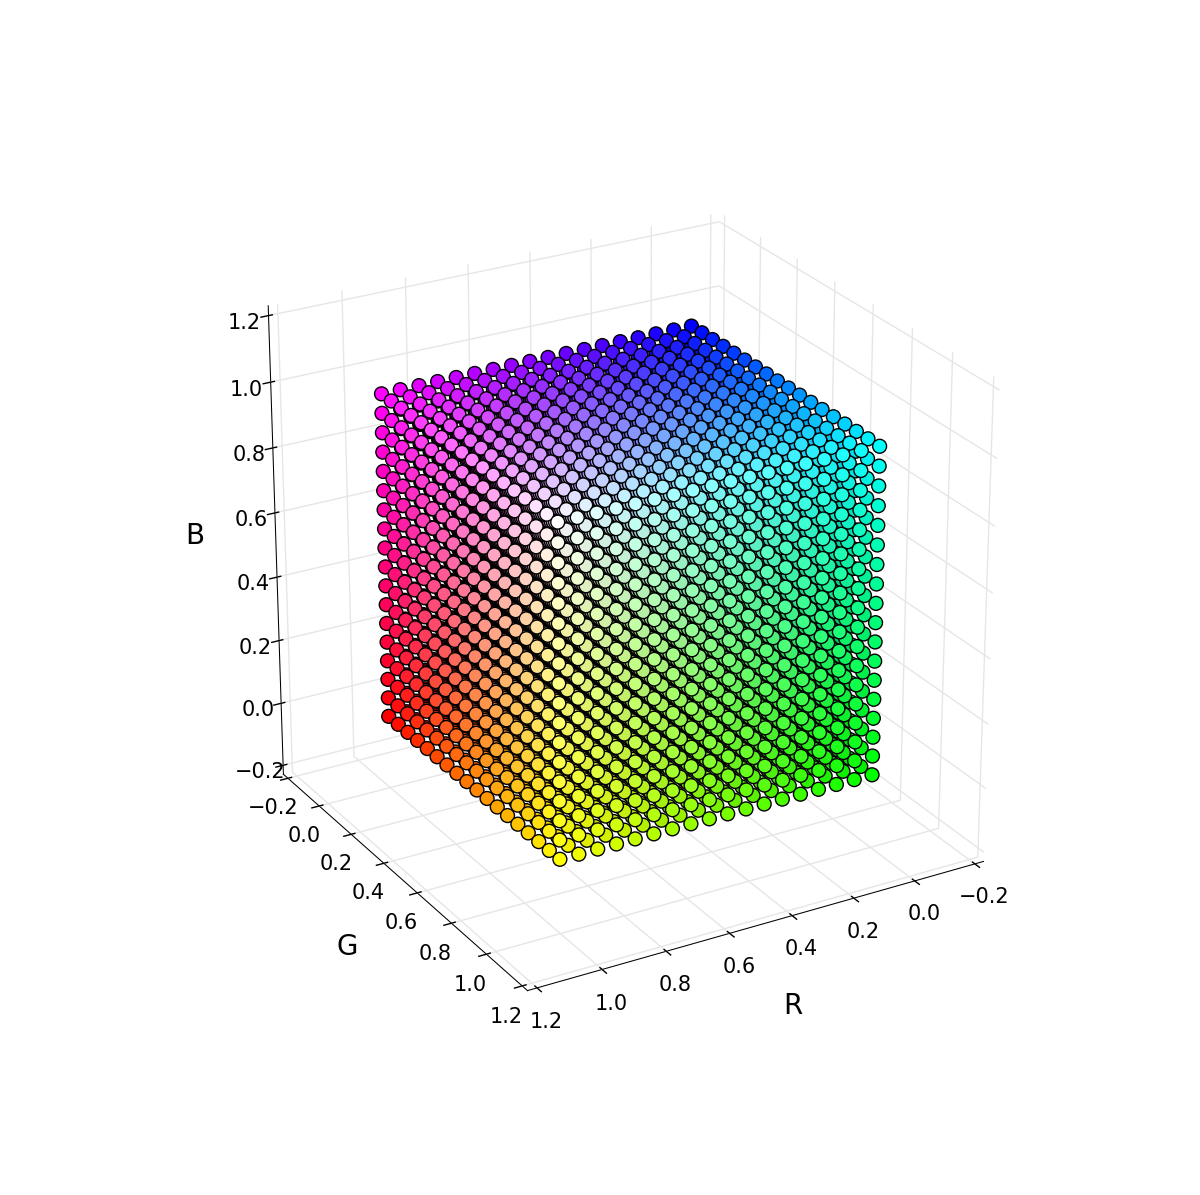
\includegraphics[width=\textwidth,trim={125px 75px 125px 75px},clip]{RGB}
		\caption{The RGB colorspace}
		\label{fig:RGB}
	\end{subfigure}
	~ %add desired spacing between images, e. g. ~, \quad, \qquad, \hfill etc. 
	%(or a blank line to force the subfigure onto a new line)
	\begin{subfigure}[b]{0.32\textwidth}
		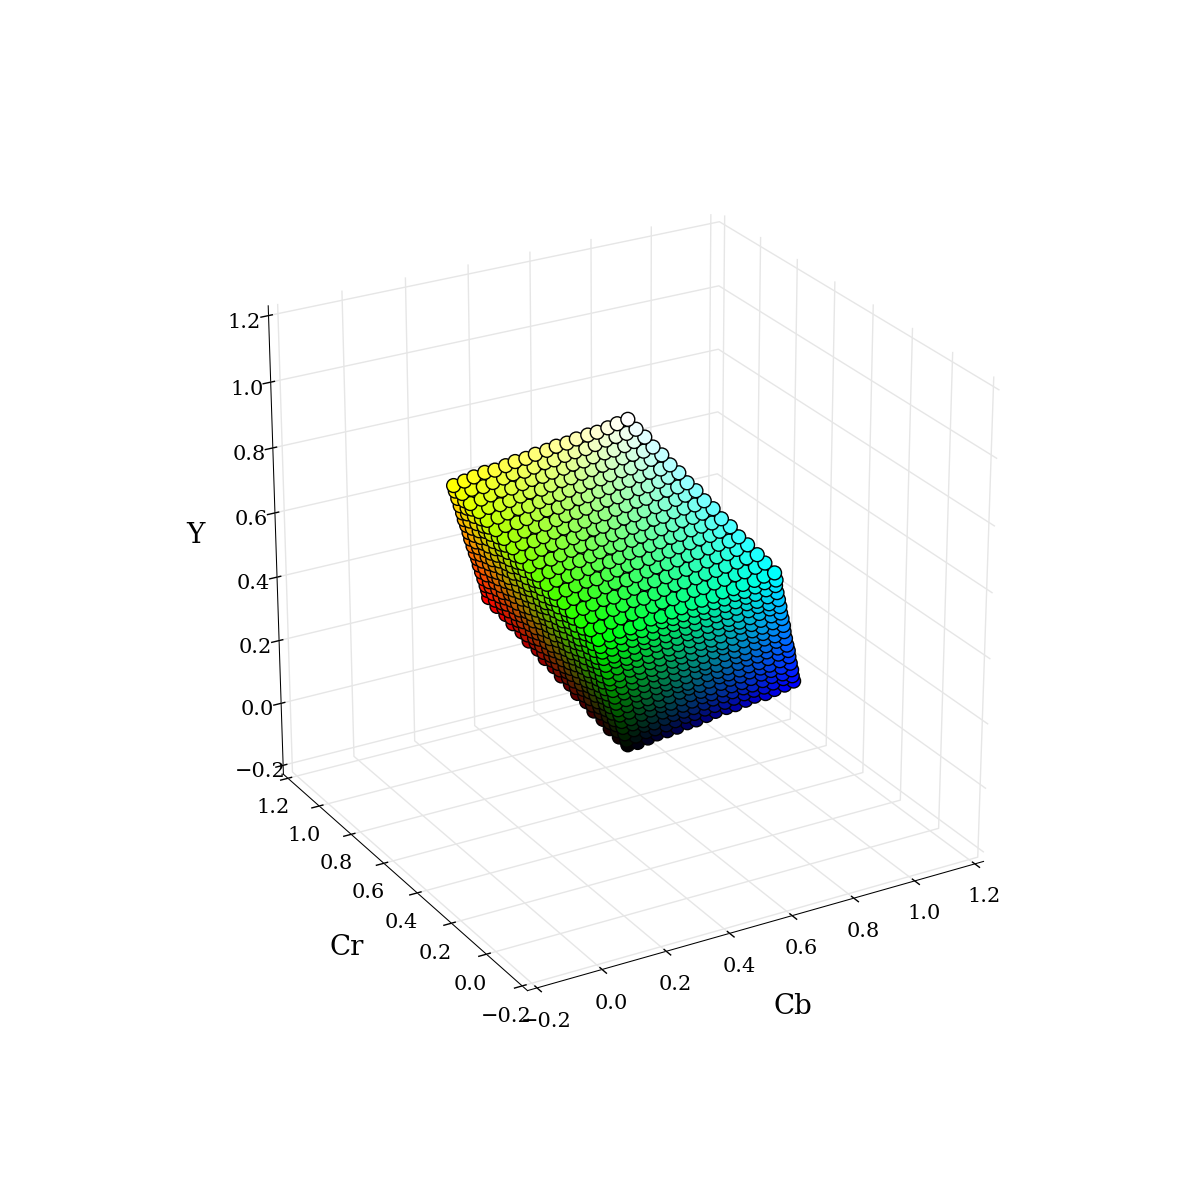
\includegraphics[width=\textwidth,trim={125px 75px 125px 75px},clip]{YCbCr}
		\caption{The RGB colorspace represented in the YCbCr colorspace}
		\label{fig:YCbCr}
	\end{subfigure}
	~ %add desired spacing between images, e. g. ~, \quad, \qquad, \hfill etc. 
	%(or a blank line to force the subfigure onto a new line)
	\begin{subfigure}[b]{0.32\textwidth}
		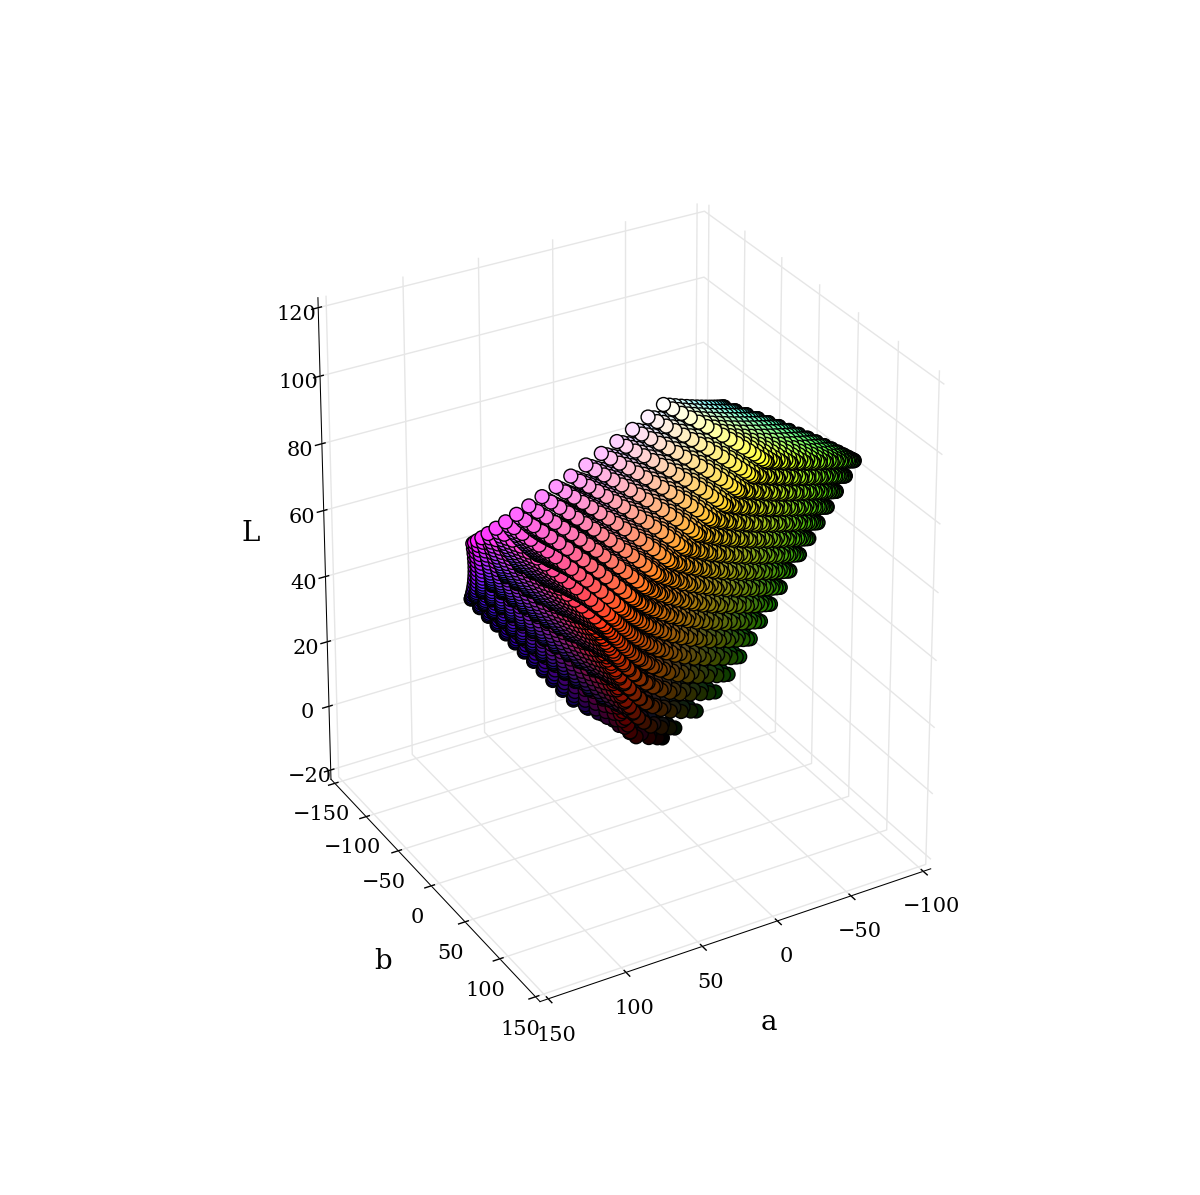
\includegraphics[width=\textwidth,trim={175px 75px 150px 75px},clip]{CIELab}
		\caption{The RGB colorspace represented in the CIELab colorspace}
		\label{fig:CIELab}
	\end{subfigure}
	\caption{The different colorspaces used in the different networks}\label{fig:animals}
\end{figure}


\subsubsection{CNN properties}
\label{sec:nnproperties}
CNNs contain a vast amount of properties to determine the networks behaviour. Most of these properties are chosen for optimum performance and a fair comparison between networks

% Throughout the report some of these parameters are kept constant for each network architecture. 

%The incoming pipeline of the CNN can be chosen to be initialed from scratch, or to be initialed with pre-trained weights. For example VGG16 \cite{Simonyan} has shown excellent results in image classification, and therefore already has a large amount of feature extraction already available.

When using a network without pre-trained weights, the networks weights have to be initialized. This is done using a Glorot Uniform distribution \cite{Glorot} as initialization of the weights. This weight initialization method samples from a uniform distribution with its variance scaled depending on the ingoing and outgoing data. %?

The intermediate layers of the network consist mainly of convolutional layers. All convolutional layers, except some output layers, use ReLu  non-linearities \cite{nair2010rectified}. 
Kernel sizes in the convolutional layers of the network are 3x3 kernels. This kernel size is based upon VGG16's \cite{Simonyan} kernel size.
Stride in the convolutional layers is 1 by default. However, in the CNNs using dilation in the output pipeline, {\color{red} ref(XXX)} stride is used as a way to downsample the resolution of the image, comparable to the function of max pooling, but remaining more spatial properties of the input image. %?
Padding is required when using convolutional layers due to the fact that border information of the image is lost when convolving. This property is set to keep the output resolution the same as the input resolution. Zero padding is used when conventional convolutions operations are performed. Symmetric padding is used when dilated convolutions are used, again the amount of padding is chosen to keep the output dimensions the same.


\subsection{Feature Extraction}
To be able to recognize certain objects in grayscale images, object dependent features are extracted. 
This is done in the first part of the convolutional neural network, up until the bottleneck of the network.
To extract these features convolutional layers are used with a varying amount of feature maps. A part of this feature extraction is reducing local features to more global features, making them invariant to spatial transformations. To accomplish this, Max-pooling is widely used. Another technique available is using an appropriate amount of stride when convolving. {\color{red}reference??}.

This results in feature maps in the bottleneck which are spatially invariant to the input. These feature maps identify for a large part what is in the image, but have a decreased amount of spatial information. To retrieve this spatial information, proper reconstruction of the image has to be done. This is expanded upon in section \ref{sec:reconstruction}.

\subsection{reconstruction}
Before the bottleneck, the image is reduced to a set of features, containing decreased amounts of spatial information. To be able to colorize the image, spatial locations of the object are required. For reconstruction, various methods are used to retrieve the original image resolution.

First of all, the feature maps can be upscaled using linear upscaling. However, to retrieve the original image not only the features but also the localisation of the features needs to be done. There are multiple ways of retrieving the spatial information of the image \cite{Charpiat} \cite{Zhang}. The methods tested in these paper consist of residual autoencoders and dilated convolutions \cite{yu2015multi}.

The use of a residual autoencoder has been demonstrated by \cite{Dahl}. After the bottleneck of the CNN each layer is upscaled and concatenated with the parralel layer in the input pipeline of the network. This way global features are merged with the localisation of those featues. This process is repeated after each upscale layer untill the output of the network is reached, as can be seen in figure \ref{fig:dahlnetwork}.

%This is done by concatenating the layers of the same resolution before the bottleneck with the upscaled features after the bottleneck. Then an convolutional layer is used to merge these features in feature maps of the upscaled resolution. This process is repeated until the original image resolution is retrieved.
%
Another technique used is the use of dilated convolutions \cite{yu2015multi}. Zhang et al. use strides in the incoming pipeline of the CNN, which causes less loss of spatial information. The bottleneck of the network consists of 28x28 feature maps. The output pipeline of the network is initialised by two layers of dilated convolutions, where each layer consists of 3 consecutive dilated convolutions. Using dilated convolutions has the effect that the input pipeline can compress the image to a larger size leaving more spatial information in the bottleneck of the image. The receptive field of dilate

\subsection{Color Generation}
In the final layers of the network, the original image color layers have to be reconstructed. Two different methods are used throughout the paper: construction using two feature maps and classification.

The construction using two feature maps is a direct result of retrieving the original image resolution through the reconstruction of the image. As a final layer, a convolutional layer is used that maps to two feature maps, which represent the two color layers that are finally used to create a colorized image.

As an aid to the colorization process, a Gaussian Blur is used on the color layers of the original image. Colorization does not require precise pixel by pixel colorization, because colors in images mostly appear in sets of pixels. When blurring, this enables the network to more easily converge towards a solution by reducing the noise in the color of the pixel set. Note that blurring the color layers does not reduce the image fidelity. This is due to the fact that the luminosity layer contains the details and contrast of the image, which is subsequently merged with the output color layers of the network. This makes the colorization problem into a regression problem, where a continuous function is sought which maps a grayscale input to the two values that determine color in the output.

The other method used is a classification approach to colorization: for a given input image, every pixel in the output image falls within one of many predefined color classes. Every color class contains a range of similar colors, where the range is smaller with a larger number of classes. While in the target image every output pixel falls into exactly one color class (the class of the actual color), classification using a neural network gives a probability distribution over the possible color classes for every pixel. This more closely resembles the nature of the colorization problem, since not every object is linked to a single color, but rather a distribution of possible colors. The final colorized version of the image is created by processing the probability distribution per pixel. Implementing an annealed mean to pick the best color from the probability distribution allows setting the degree with which to pick either the mode or the mean of the distribution.

Both the two feature maps and classification approach are tried during the present research.



\subsection{Loss Function}
The loss function depends on the network architecture. In this paper roughly two different types of networks are used;Two feature maps output and classification. 

The two feature maps represent the color space layers of the to be reconstructed image, depending on the selected colorspace. The loss function is then defined as the sum squared distance between the output of the network and the original image color layers. This can be seen in equation \ref{eq:squaredsum}, where $p$ is the prediction of the network and $t$ is the target. 

\begin{equation}
\label{eq:squaredsum}
L = (p - t)^2
\end{equation}

To enable the network to use more saturated colors, color rebalancing is applied to the loss function. This color rebalancing penalized the the network for selecting desaturated colors, by exponentially increasing the loss function when converging towards desaturated solutions. However, this did not produce desired results, due to the fact that it was figure dependend and difficult to tune to a global solution. 

For classification, categorical cross-entropy is used. This is done between the predicted color classification of the network per pixel and the target classification per pixel of color layers of the image. The categorical cross-entropy function is defined in equation \ref{eq:crossentropy}, where $t_{i,j}$ is the target classification. $t_i$ stands for each pixel, where $t_j$ stands for its respective probability distribution of the classified color. 
$p_{i,j}$ is the predicted classification, where $p_{i}$ depicts the predicted pixel. $p_{j}$ is the estimated probability distribution of the classified color, by the network.  

\begin{equation}
\label{eq:crossentropy}
L_{i} = -\sum t_{i,j}\log(p_{i,j})
\end{equation}

The distribution of colors in the dataset is strongly biased towards desaturated colors. For classification, class rebalancing was added to assist the network in selecting more saturated colors. This was done by generating a histogram of the discrete colors in the dataset and using this information to balance out the loss function with respect to each color. This histogram is then merged with a uniform distribution($\lambda$) as hyper parameter to set the intensity of the color rebalancing. To keep the color rebalancing within reasonable bounds, its expected value is kept equal to one. Equation \ref{eq:classrebalance} is the applied class rebalancing, where $V$ is the class rebalance output, $H$ is the dataset histogram and $\lambda$ is the uniform distribution. 

\begin{equation}
V = ((1 - \lambda)\cdot H + \lambda)^{-1}
\end{equation}
 
\subsection{Model Architectures}
A major part in creating a successful neural network is finding a suitable network architecture. For image classification convolutional neural networks are widely used with success \cite{Krizhevsky,Szegedy,Simonyan}. For our purpose a main feature of the convolutional network is that the image has to be reconstructed again, to retrieve spatial information.

{\color{red} 
In total a set of three convolutional network architectures are used. An architecture based upon Dahl \cite{Dahl}, a pre-trained VGG16 \cite{Simonyan} architecture {\color{red} this is actually Dahl,  not sure about the actual amount of layers used for the reconstruction} and a classification architecture \cite{Zhang}. The architectures of the network are split up in a feature extraction part and a reconstruction part, which will be expanded upon in the following sections.}\\ 
\\%weet neit of je dit mag zeggen..

{\color{red}
\textbf{Feature extraction}

%%Check op diepgang.

\subsubsection{Dahl}%weet geen naam}


This convolutional network is based upon the architecture used by Dahl \cite{Dahl}. It contains several convolutional layers, which use a 3x3 kernel throughout the network. After a set of convolutions a batch normalization is done followed by a max pool layer. Batch normalization is added such that in the reconstruction of the image the concatenated layers are in the same order of magnitude. The architecture was modified to fit the input dimensions. The network is an untrained network, having Glorit uniform distributed \cite{Glorot} initialized weights, meant to be trained simultaneously with the rest of the network. At the bottleneck of the architecture, the resolution of the feature maps are reduced to 16x16 pixels.
 
%Figure toevoegen van het netwerk

\subsubsection{VGG16}
A substantial amount of pre-trained networks are available, trained on the ImageNet classification database. The architecture used is based upon VGG16 \cite{Simonyan}, which uses a 3x3 kernel throughout the network. This network has a proven architecture, and can be obtained with pre-trained weights. Modifications on the network where required to fit the input dimensions. VGG16 is used in classification of RGB images, while our network only needs one input, a grayscale image. The pre-trained weights of the three input maps where averaged to accept a single grayscale input image. The VGG16 architecture features several convolutional layers followed by max pooling. Batch normalization was added before every max pool layer, such that in the later concatenation of the layers the values are in the same order of magnitude. At the bottleneck of the architecture the feature maps have a resolution of 16x16 pixels. 

\subsubsection{Classification}
The classification architecture shares much similarities with the VGG16 architecture. The main difference can be found in the final layers of the network. This is due to the fact that classification is used rather than direct reconstruction of the wanted color layers. This classification is subsequently used to colorize the image. \\
\\
\textbf{Reconstruction}

For reconstruction of the image, linear up-scaling is used. The reconstruction begins after the bottleneck of the convolutional network is reached, where the resolution of the feature maps is 16x16 pixels. The up-scaled information is concatenated with the convolutional layer before the bottleneck that matches the up-scaled layer resolution. Then a convolutional layer is used for feature extraction of the concatenated layer. A batch normalization is applied and the processes is repeated until the original image resolution is retrieved. For both the VGG16 and Dahl based architecture a final output layer is used with a 2 feature map output, which match to the corresponding colour output layers.

For the classification the image is reconstructed to its original resolution. However, first a convolutional layer using a 1x1 kernel is used that has the same amount of feature maps as the required number of possible color classification bins. Then, these feature maps, representing discretized colours, %jopie jou expertise.


A detailed representation with of the various architectures is given in figure {\color{red}(XXX)}}

\subsection{Loss function}

\begin{wrapfigure}{R}{0.5\textwidth}
	\vspace{-20pt}
	\begin{center}
		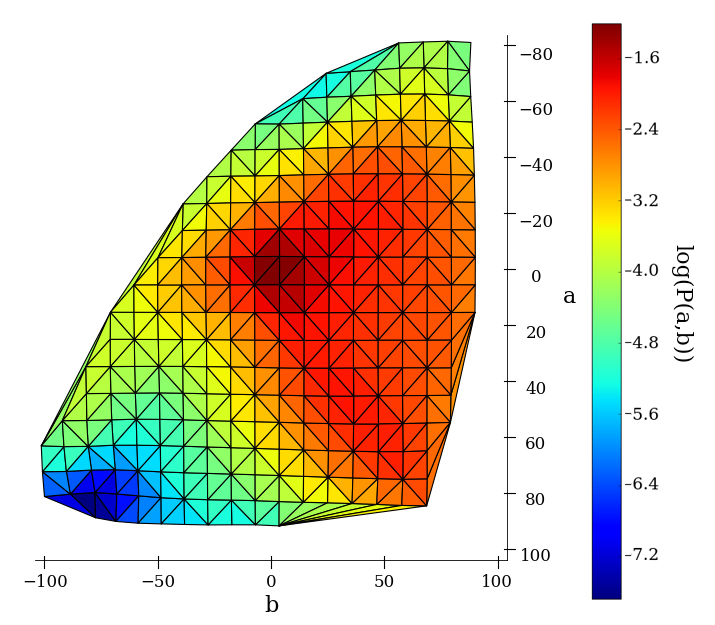
\includegraphics[width=0.48\textwidth]{hist}
	\end{center}
	\caption{\color{red} The histogram of the total fruit dataset}
	\vspace{-10pt}
\end{wrapfigure}

\subsection{Training method}
For convolutional neural networks stochastic gradient decent {\color{red}(SGD)}, sometimes together with momentum, is commonly used for updating the weights and biases \cite{IizukaSIGGRAPH2016} \cite{Simonyan}. The used hyper-parameters, especially the learning rate, requires careful tuning when using SGD. Often scheduled learning rate, that is monotonically decreasing depending on the epoch, results in the best results. 




\section{Results}\label{sec:results}
%Results
%Show effect of colorspaces, blur, annealed mean
%Compare results of architectures (images, error plot, feature maps)

In section \ref{sec:


\section{Discussion}

Defining a quantitative performance measure of the networks is outside of the scope of this paper. Therefore a comparison of the results of the five architectures is mainly done by sight.

%comparison of datasets fruit and landscape, on compact net . 
\subsection{Comparing datasets}
The compact network is the only network that was trained on both the landscape dataset and the fruit dataset. In figure \ref{fig:blur} the final results after 25 epochs on the landscape dataset can be seen. The algorithm seems to color landscapes to good standards. However it is concluded that landscape datasets offer less strain on the CNN, because landscapes contain only a small set of features coupled to colors. For example, trees, sea and grass cover a large amount of the landscape dataset, as opposed to the many classes of fruit in the fruit-dataset. In addition, images of landscapes offer a very low amount of spatial transformation. Strawberries and bananas come in many orientations and shapes, whereas landscapes always have a horizon where the top part is blue and the bottom part is green or brown. Therefore the landscape dataset is labeled to be a low-level test-case of the CNNs, and the fruit-dataset is used as a better performance measure for the CNNs.

%discussion on difference between YcbYcr and Cielab Effect of blur
\subsection{Comparing colorspace and effect of blur}
The only network using regression was the Compact network. Gaussian blur is used to allow the network to more easily converge towards a solution. Different kernel sizes for Gaussian blur are used, $\sigma = 0$, $\sigma = 3$ and $\sigma = 5$ which can be seen in figure \ref{fig:blur}. Using $\sigma = 0 $ results in a sepia/grayscale image. 
Clearly the network is having difficulties with convergence towards an optimal solution. Without blurring, the target data will be noisy, and thus there will be more local minima and maxima in the loss function hyperspace. This is why sepia/grayscale is an appropriate solution when not blurring. $\sigma = 3$ and $\sigma = 5$ show promising results. The difference between both pictures is marginal, however a higher $\sigma$ will result in an average color overlay, on the landscape set the whole image has a blue tint. This is why $\sigma = 3$ is chosen as optimal setting.


As for colorspace selection, a comparison is made on the Compact network that shows difference between the YCbCr and CIELab colorspaces. CIELab shows a marginal improvement in saturation compared to YCbCr. This result is indecisive for making a decision on the best colorspace. However, CIELab has the added benefit that a certain color is independent of the Luminosity. This means that, when the CIELab space is divided into bins for the classification, each bin can represent a specific color, only changing in luminosity depending on the value of the added L layer. This is why CIELab is chosen as colorspace for the classification architectures.


%overfitting of vgg16 so dataset too small
% using compact architectures better results
\subsection{Comparing network complexity}
Another aspect that can be noted is that Networks are prone to overfitting on the small dataset that is used. The fruit dataset consisted of 6000 unique images for training and 1000 images for validation, both doubled in size by mirroring them. The most complex network is the VGG16 + classification network. This architecture has 512 feature maps in the bottleneck of the network. As can be seen in \ref{fig:overfit}, the VGG16 + classification network is evidently overfitting after 10 epoch. {\color{red} hier mag wel iets meer tekst?}


%comparison between dilation, concat and dilation+concat
\subsection{Comparing feature localization}
As can be seen in figure \ref{fig:results}, most of the architectures offer a satisfactory performance of the fruit dataset. However interesting differences can be seen in this comparison. For example the effect of class-rebalancing is very evident between the regression and classification networks. Class-rebalancing was implemented on all the classification networks with a $\lambda$ of 0.3, except for the VGG16 classifier where $\lambda = 0.5$. The images in the classification networks offer more vibrant colors, where the colors in the regression network are more dull. The fruit dataset is biased towards green red and especially gray colors, as can be seen in figure \ref{fig:histogram}. Class-rebancing therefore offers a good solution to add in more exotic colors in the images which are less common in the dataset.

Interesting to notice, is the difference between the dilated and concatenated networks. It can be seen that the networks sometimes still has difficulty with the correct localization of the color. Both the dilated and the concatenated networks show a substantial amount of color artifacts in the output image. For example, the middle image, in figure \ref{fig:results}, consisting of the fruit bowl, both networks color a part of the kiwi red. This originates from the red used in the neighboring strawberry, the network is not accurate enough in localization of the strawberry. However a difference can be noted between the two configurations: the dilated version shows less artifacts then the concatenated networks. An explanation could be that the network gets steered to the correct colors already by mapping the grayscale value to a reduced set of colors. For example, the image with strawberries in the second picture in appendix \ref{ap:more_results}, shows a strawberry colored green. However the network has no idea whether this strawberry needs to be colored green or red, still it picks the color green. All the five networks show this behavior, this is some evidence that the network uses some of the information in the grayscale input values to map a color to the image. The concatenated network use a lot more of this information since the input layers are concatenated with the output pipeline. Thus instead of picking a 'realistic' color, the concatenated network maps more of the input information in the outline pipeline of the network, hence often creating objects that are partially colored with the ground truth color, as can be seen in the fifth row of the figure in appendix \ref{ap:more_results}. In most images, the dilated convolution network results in a more realistic coloring then the network using concatenation. However the dilated network often has difficulty in coloring images which contain a large variety of small pieces of fruit, as can be seen in the seventh row in appendix \ref{ap:more_results}.

%final comparison between all architectures, show massive image.
\subsection{Final comparison}

%conclusion on best network







%Gaussian blur
%It is clear that the case with $\sigma=0$, i.e. no blur, the network was unable to find any colors. Using a blur radius of $\sigma=3$ or $\sigma=5$ leads to much better results. Between these two, the $\sigma=3$ case was chosen to be the best, since it seems more inclined to pick more saturated colors. A too high blur radius will also make the training less effective since the link between texture and color becomes weaker at the edges of objects.
\section{Conclusion}


Conclusion


\section{Recommendations}

Recommendations: What's next
hyperparameters research (momentum etc)
longer training
bigger training set
extend usage to all images
\section{Recommendations}

%Recommendations: What's next
%hyperparameters research (momentum etc)
%longer training
%bigger training set
%extend usage to all images

\FloatBarrier
\bibliography{./Bibliography/Bibliography}
\bibliographystyle{ieeetr}


\newpage
\appendices
\section{Neural network settings}\label{ap:NNset}
\begin{table}[h]
	\centering
	\caption{Parameters of the compared architectures.\label{tab:architectures}}
	\footnotesize
	\begin{tabular}{|l|l|l|l|l|l|}
		\hline
		& \textbf{compact}                                                  & \textbf{compact classifier}                                       & \textbf{\begin{tabular}[c]{@{}l@{}}compact classifier\\  dilated\end{tabular}}                             & \textbf{\begin{tabular}[c]{@{}l@{}}compact classifier\\  dilated + concat\end{tabular}} & \textbf{\begin{tabular}[c]{@{}l@{}}vgg16 \\ + classifier\end{tabular}} \\ \hline \hline
		\multicolumn{6}{|l|}{\textbf{dataset parameters}} \\ \hline
		\textit{Color space}               &   YCbCr and CIELab           &   CIELab        &        CIELab                      &         CIELab                       &     CIELab                                      \\ \hline
		\textit{Fruit dataset}             & Yes                                                               & Yes                                                               & Yes                                                               & Yes                                                                                      & Yes                                                                            \\ \hline
		\textit{Landscape dataset}         & Yes                                                               & No                                                                & No                                                                & No                                                                                       & No                                                                             \\ \hline \hline
		\multicolumn{6}{|l|}{\textbf{Hyperparameter}} \\ \hline 
		\textit{Training method}           & \begin{tabular}[c]{@{}l@{}}ADADELTA\\  with momentum\end{tabular} & \begin{tabular}[c]{@{}l@{}}ADADELTA\\  with momentum\end{tabular} & \begin{tabular}[c]{@{}l@{}}ADADELTA\\  with momentum\end{tabular} & \begin{tabular}[c]{@{}l@{}}ADADELTA with \\ momentum\end{tabular}                        & \begin{tabular}[c]{@{}l@{}}ADADELTA\\  with momentum\end{tabular}              \\ \hline
		\textit{Epochs trained}            &     50       &     28  &     30   &     30                                                                                     &      25                                                                          \\ \hline
		\textit{Batch size}                &         20                                                          &     20                                                              &       20                                                            &        20                                                                                  &   20                                                                            \\ \hline \hline
		\multicolumn{6}{|l|}{\textbf{Architecture properties}} \\ \hline 
		\textit{Front end module}          & trained from scratch                                              & trained from scratch                                              & trained from scratch                                              & trained from scratch                                                                     & VGG16 front end                                                                \\ \hline
		\textit{Max pool}                  & Yes                                                               & Yes                                                               & No                                                                & No                                                                                       & Yes                                                                            \\ \hline
		\textit{Strides}                   & No                                                                & No                                                                & Yes                                                               & Yes                                                                                      & No                                                                             \\ \hline
		\textit{dilation}                  & No                                                                & No                                                                & Yes                                                               & Yes                                                                                      & No                                                                             \\ \hline
		\textit{Concatenation}             & Yes                                                               & Yes                                                               & No                                                                & Yes                                                                                      & Yes                                                                            \\ \hline
		\textit{Kernel size}               & 3x3                                                               & 3x3                                                               & 3x3                                                               & 3x3                                                                                      & 3x3                                                                            \\ \hline
		\textit{Activation function}       & ReLu                                                              & ReLu                                                              & ReLu                                                              & ReLu                                                                                     & ReLu                                                                           \\ \hline
		\textit{Batch norm}                & Yes                                                               & Yes                                                               & Yes                                                               & Yes                                                                                      & Yes                                                                            \\ \hline \hline
		\multicolumn{6}{|l|}{\textbf{Classification properties}} \\ \hline  
		\textit{Annealed mean temperature} & 0.4                                                                   &0.4                                                                   &0.4                                                                   &0.4                                                                                          &0.4                                                                                \\ \hline
		\textit{K-nearest neighbour}       & -                                                                 & 10                                                                & 10                                                                & 10                                                                                       & 10                                                                             \\ \hline
		\textit{K-nearest neighbour sigma} & -                                                                 & 5                                                                 & 5                                                                 & 5                                                                                        & 5                                                                              \\ \hline
		\textit{Number of colorbins} & -                                                                 & 247                                                                 & 247                                                                 & 247                                                                                        & 247                                                                              \\ \hline
		\textit{Uniform mixing factor ($\lambda$)} & -                                                                 & 0.3                                                                 & 0.3                                                                 & 0.3                                                                                        & 0.5                                                                              \\ \hline
	\end{tabular}
\end{table}

\newpage
\section{Training and validation errors}\label{ap:errors}
\begin{figure}[h]
	\centering
	\begin{subfigure}[b]{0.48\textwidth}
		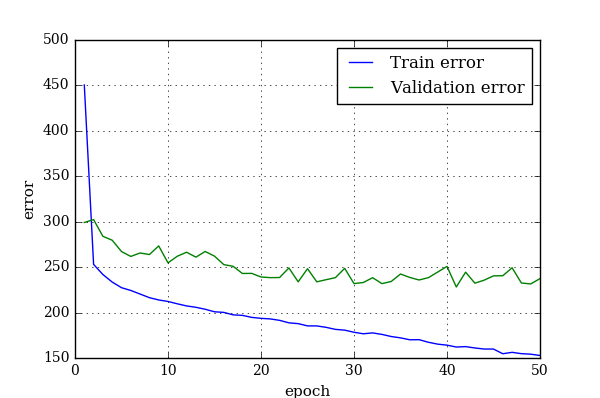
\includegraphics[width=\textwidth]{errors_fruit_Compact_more_end_fmaps_YCbCr_sigma3}
		\caption{Compact}
		\label{fig:eror_comp}
	\end{subfigure}
	\begin{subfigure}[b]{0.48\textwidth}
		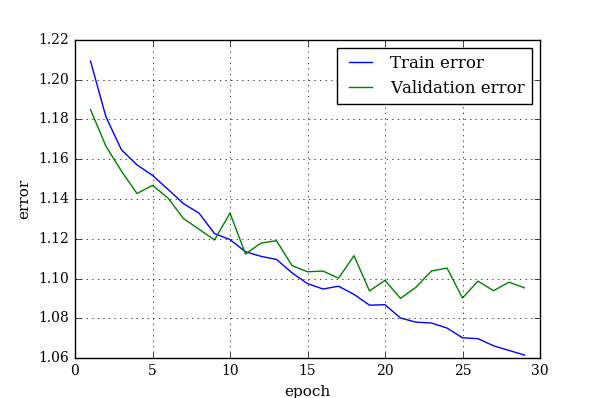
\includegraphics[width=\textwidth]{errors_fruit_Compact_more_end_fmaps_classifier_k10_T02_sigma5_nbins20_labda_03_gridsize10}
		\caption{Compact classifier}
		\label{fig:eror_comp_class}
	\end{subfigure}
	~ %add desired spacing between images, e. g. ~, \quad, \qquad, \hfill etc. 
	%(or a blank line to force the subfigure onto a new line)
	\begin{subfigure}[b]{0.48\textwidth}
		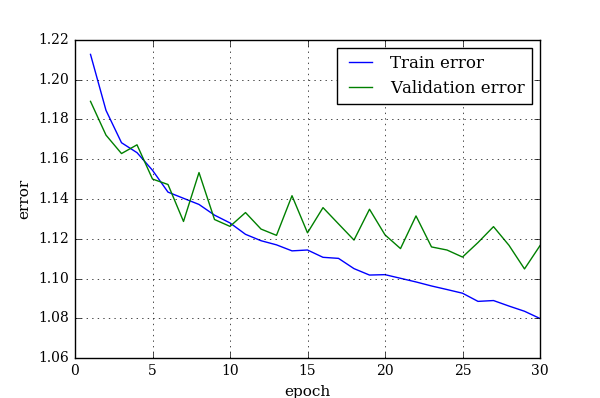
\includegraphics[width=\textwidth]{errors_fruit_Compact_more_end_fmaps_dilation_concat_k10_T02_sigma5_nbins20_labda_03_gridsize10.png}
		\caption{Compact classifier dilation + concat}
		\label{fig:error_comp_class_dila_con}
	\end{subfigure}
	~ %add desired spacing between images, e. g. ~, \quad, \qquad, \hfill etc. 
	%(or a blank line to force the subfigure onto a new line)
	\begin{subfigure}[b]{0.48\textwidth}
		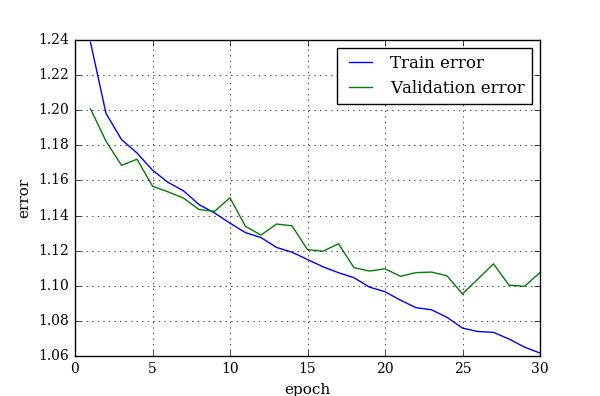
\includegraphics[width=\textwidth]{errors_fruit_Compact_more_end_fmaps_dilation_k10_T02_sigma5_nbins20_labda_03_gridsize10}
		\caption{Compact classifier dilation}
		\label{fig:error_comp_class_dila}
	\end{subfigure}
	\caption{The error plots for the different architectures. Note the large difference between the validation error and the train error for the compact architecture. That is due to the blur that is applied to the train dataset but not to the validation training set.}\label{fig:errors}
\end{figure}

\newpage
\section{More results}\label{ap:more_results}
\begin{figure}[h]
	\centering
	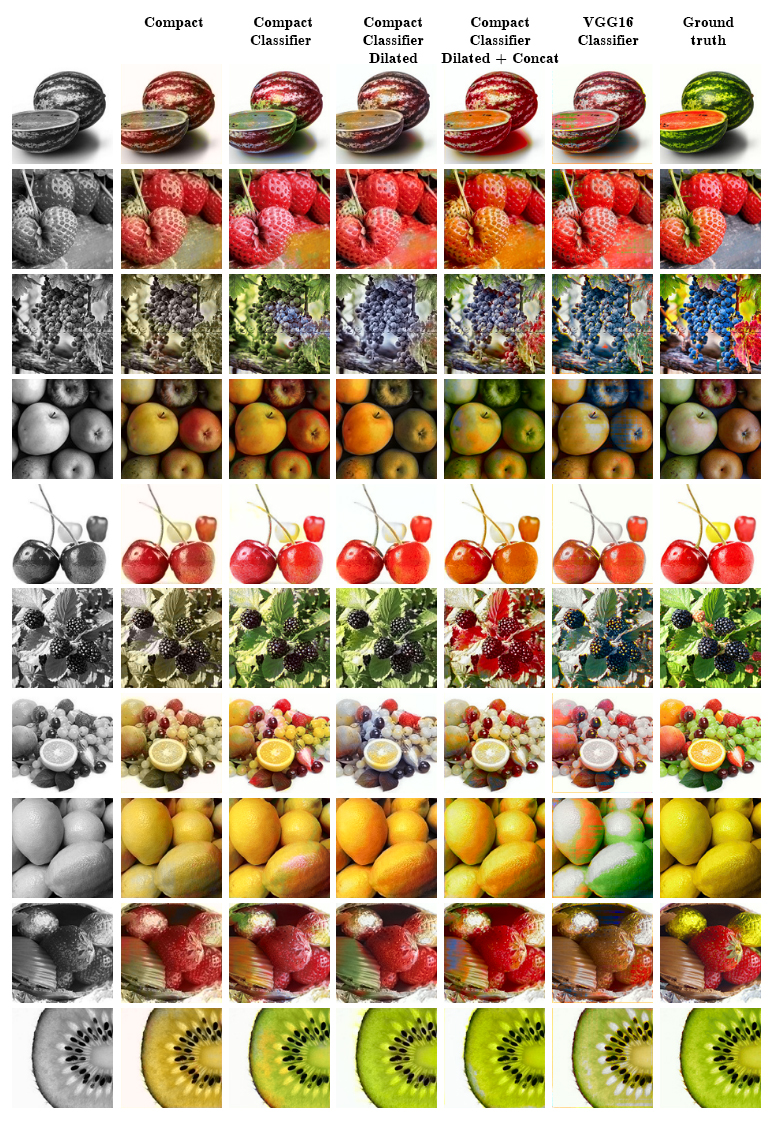
\includegraphics[width=0.83\textwidth]{set1}
	\label{fig:moreresults}
\end{figure}









 \end{document}


